\documentclass[12pt,letterpaper]{ctexart}
\usepackage{fullpage}
\usepackage[top=2cm, bottom=4.5cm, left=2.5cm, right=2.5cm]{geometry}
\usepackage{amsmath,amsthm,amsfonts,amssymb,amscd}
\usepackage{lastpage}
\usepackage{enumerate}
\usepackage[binary-units=true]{siunitx}
\usepackage{fancyhdr}
\usepackage{mathrsfs}
\usepackage{xcolor}
\usepackage{graphicx} %插入图片的宏包
\usepackage{float} %设置图片浮动位置的宏包
\usepackage{subfigure} %插入多图时用子图显示的宏包
\usepackage{listings}
\usepackage{afterpage}
\usepackage{hyperref}
\hypersetup{
    colorlinks=true,
    linkcolor=blue,
    filecolor=magenta,
    urlcolor=cyan,
}

\newcommand\blankpage{%
  \null
  \thispagestyle{empty}%
  \addtocounter{page}{-1}%
  \newpage
}


\hypersetup{%
  colorlinks=true,
  linkcolor=blue,
  linkbordercolor={0 0 1}
}

\renewcommand\lstlistingname{Algorithm}
\renewcommand\lstlistlistingname{Algorithms}
\def\lstlistingautorefname{Alg.}

\lstdefinestyle{Python}{
    language        = Python,
    frame           = lines,
    basicstyle      = \footnotesize,
    keywordstyle    = \color{blue},
    stringstyle     = \color{green},
    commentstyle    = \color{red}\ttfamily
}

\setlength{\parindent}{0.0in}
\setlength{\parskip}{0.05in}

% Edit these as appropriate
\newcommand\course{CS305}
\newcommand\hwnumber{7}                  % <-- homework number
\newcommand\NetIDa{11711918}           % <-- NetID of person #1
\newcommand\NetIDb{吴烨昌}           % <-- NetID of person #2 (Comment this line out for problem sets)

\pagestyle{fancyplain}
\headheight 35pt
\lhead{\NetIDa}
\lhead{\NetIDa\\\NetIDb}                 % <-- Comment this line out for problem sets (make sure you are person #1)
\chead{\textbf{\Large Assignment \hwnumber}}
\rhead{\course \\ \today}
\lfoot{}
\cfoot{}
\rfoot{\small\thepage}
\headsep 1.5em

\begin{document}

\section*{Problem 7.1}

{\bf Description}

Select one UDP packet from your trace. From this packet, determine
\begin{enumerate}
  \item How many fields there are in the UDP header.
  \item The name of each fields in the UDP header.
  \item The length (in bytes) of each fields in the UDP header.
  \item What is the maximum number of bytes that can be included in a UDP payload?  (Hint: the answer to this question can be determined by your answer to 3) above.)
  \item What is the largest possible source port number? (Hint: same as the hint in 4) above.)
  \item What is the protocol number for UDP? (Give your answer in both hexadecimal and decimal notation.)
\end{enumerate}


{\bf Solution}

As UDP packet captured in Figure~\ref{fig:udp}

\begin{enumerate}
  \item 4 fields.
  \item Source Port; Destination Port; Length; Checksum.
  \item 2 bytes per field.
  \item The length field is 2 bytes, has range $[0, 2^{16}-1]$. Consider that UDP header takes 8 bytes. So the maximum length is $2^{16}-1-8 = 65527$ bytes.
  \item The source port field is 2 bytes, has range $[0, 2^{16}-1]$. So the maximum source port is $65535$.
  \item 0x11 in hexadecimal, 17 in decimal.
\end{enumerate}


\begin{figure}[H]
  \centering
  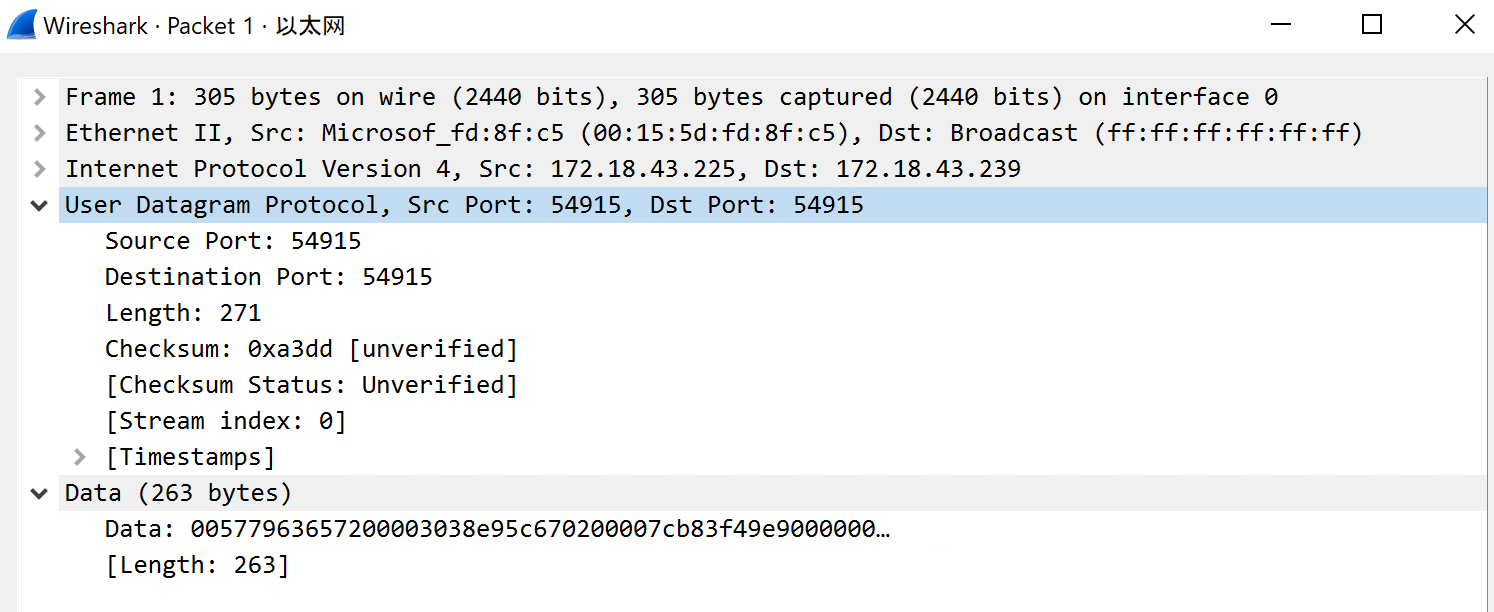
\includegraphics[width=\linewidth]{assets/udp.png}
  \caption{A UDP packet}
  \label{fig:udp}
\end{figure}

\newpage

\section*{Problem 7.2.4}

{\bf Description}

What is the sequence number of the TCP SYN segment that is used to initiate the TCP connection between the client computer and \href{gaia.cs.umass.edu}{gaia.cs.umass.edu}?
What is it in the segment that identifies the segment as a SYN segment?


{\bf Solution}

Visit \href{gaia.cs.umass.edu}{gaia.cs.umass.edu} and capture the TCP packet.

As packet captured in Figure~\ref{fig:tcp}, 0 is the sequence number. SYN segments can be told by the Syn bit set in the Flags field.

\begin{figure}[H]
  \centering
  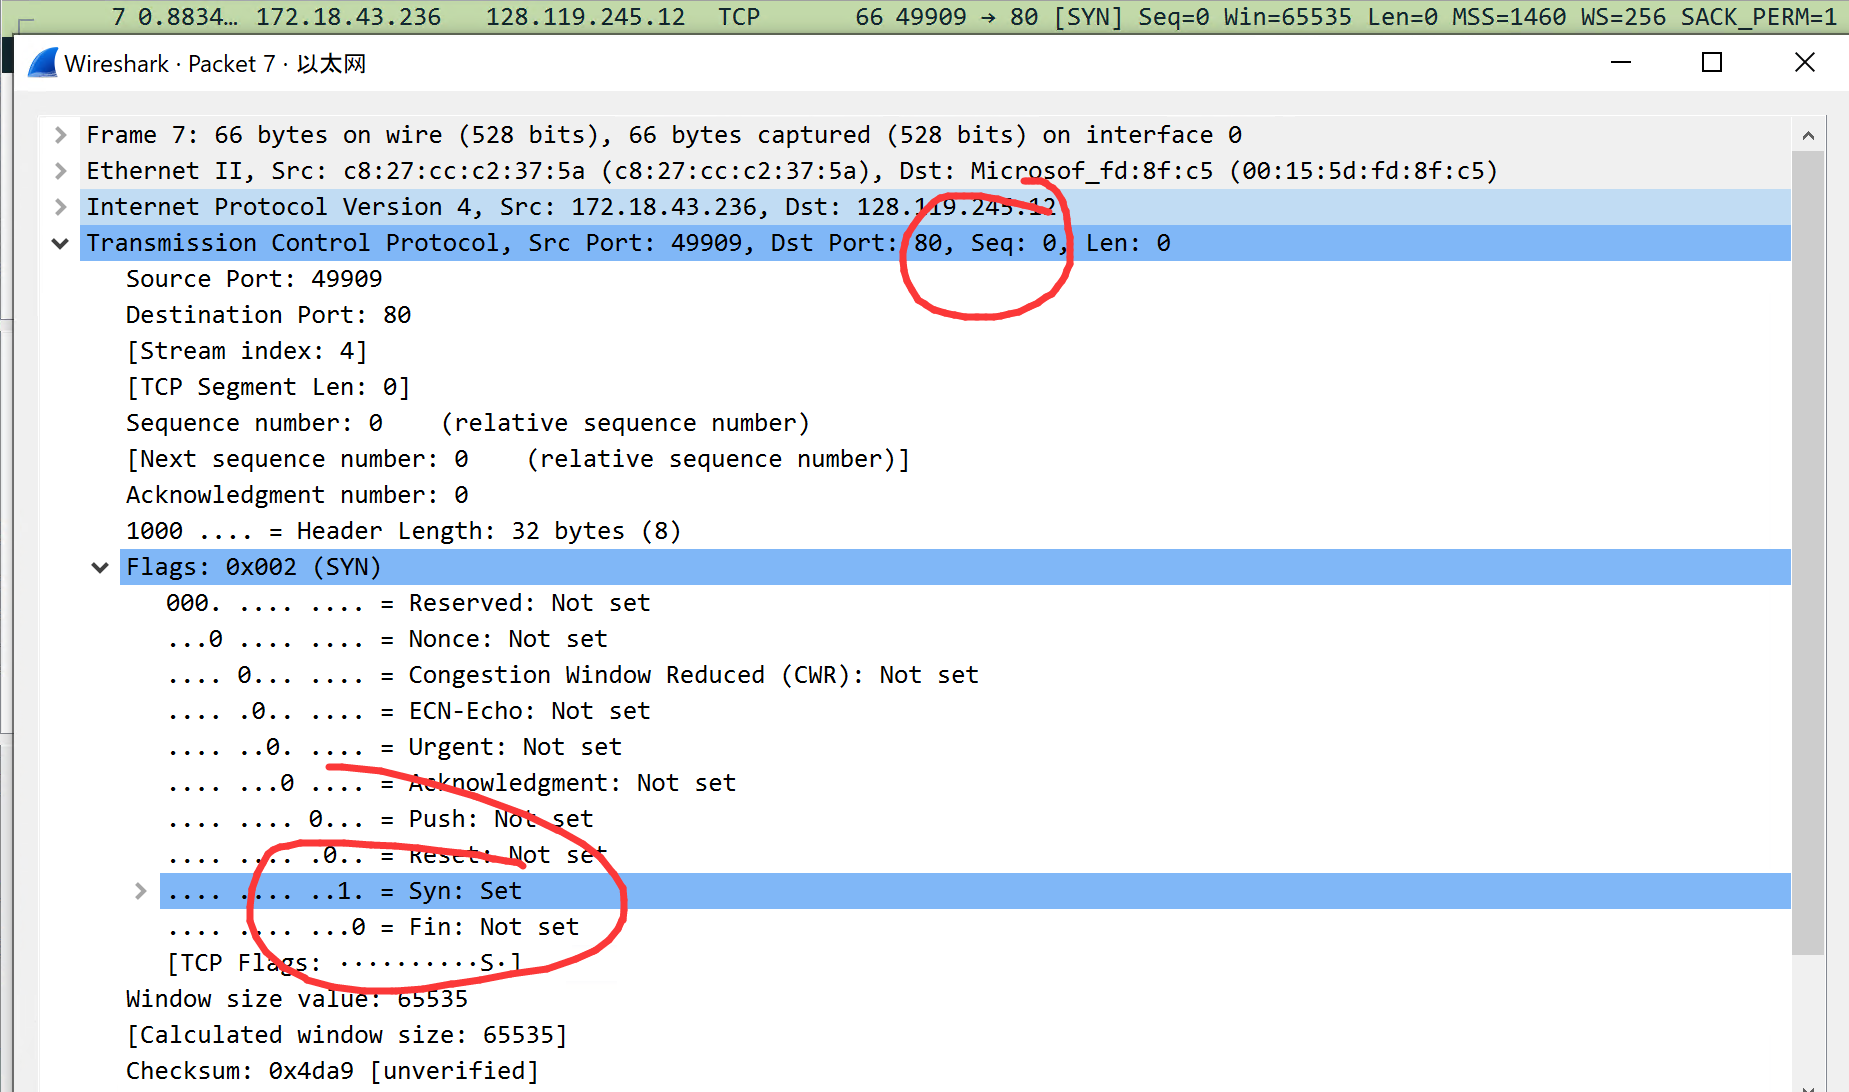
\includegraphics[width=\linewidth]{assets/tcp.png}
  \caption{TCP connection to \href{gaia.cs.umass.edu}{gaia.cs.umass.edu}}
  \label{fig:tcp}
\end{figure}

\newpage


\section*{Problem 7.2.6}

{\bf Description}

What is the sequence number of the TCP segment containing the HTTP POST command?
Note that in order to find the POST command, you’ll need to dig into the packet content field at the bottom of the Wireshark window, looking for a segment with a “POST” within its DATA field.

{\bf Solution}


\begin{figure}[H]
  \centering
  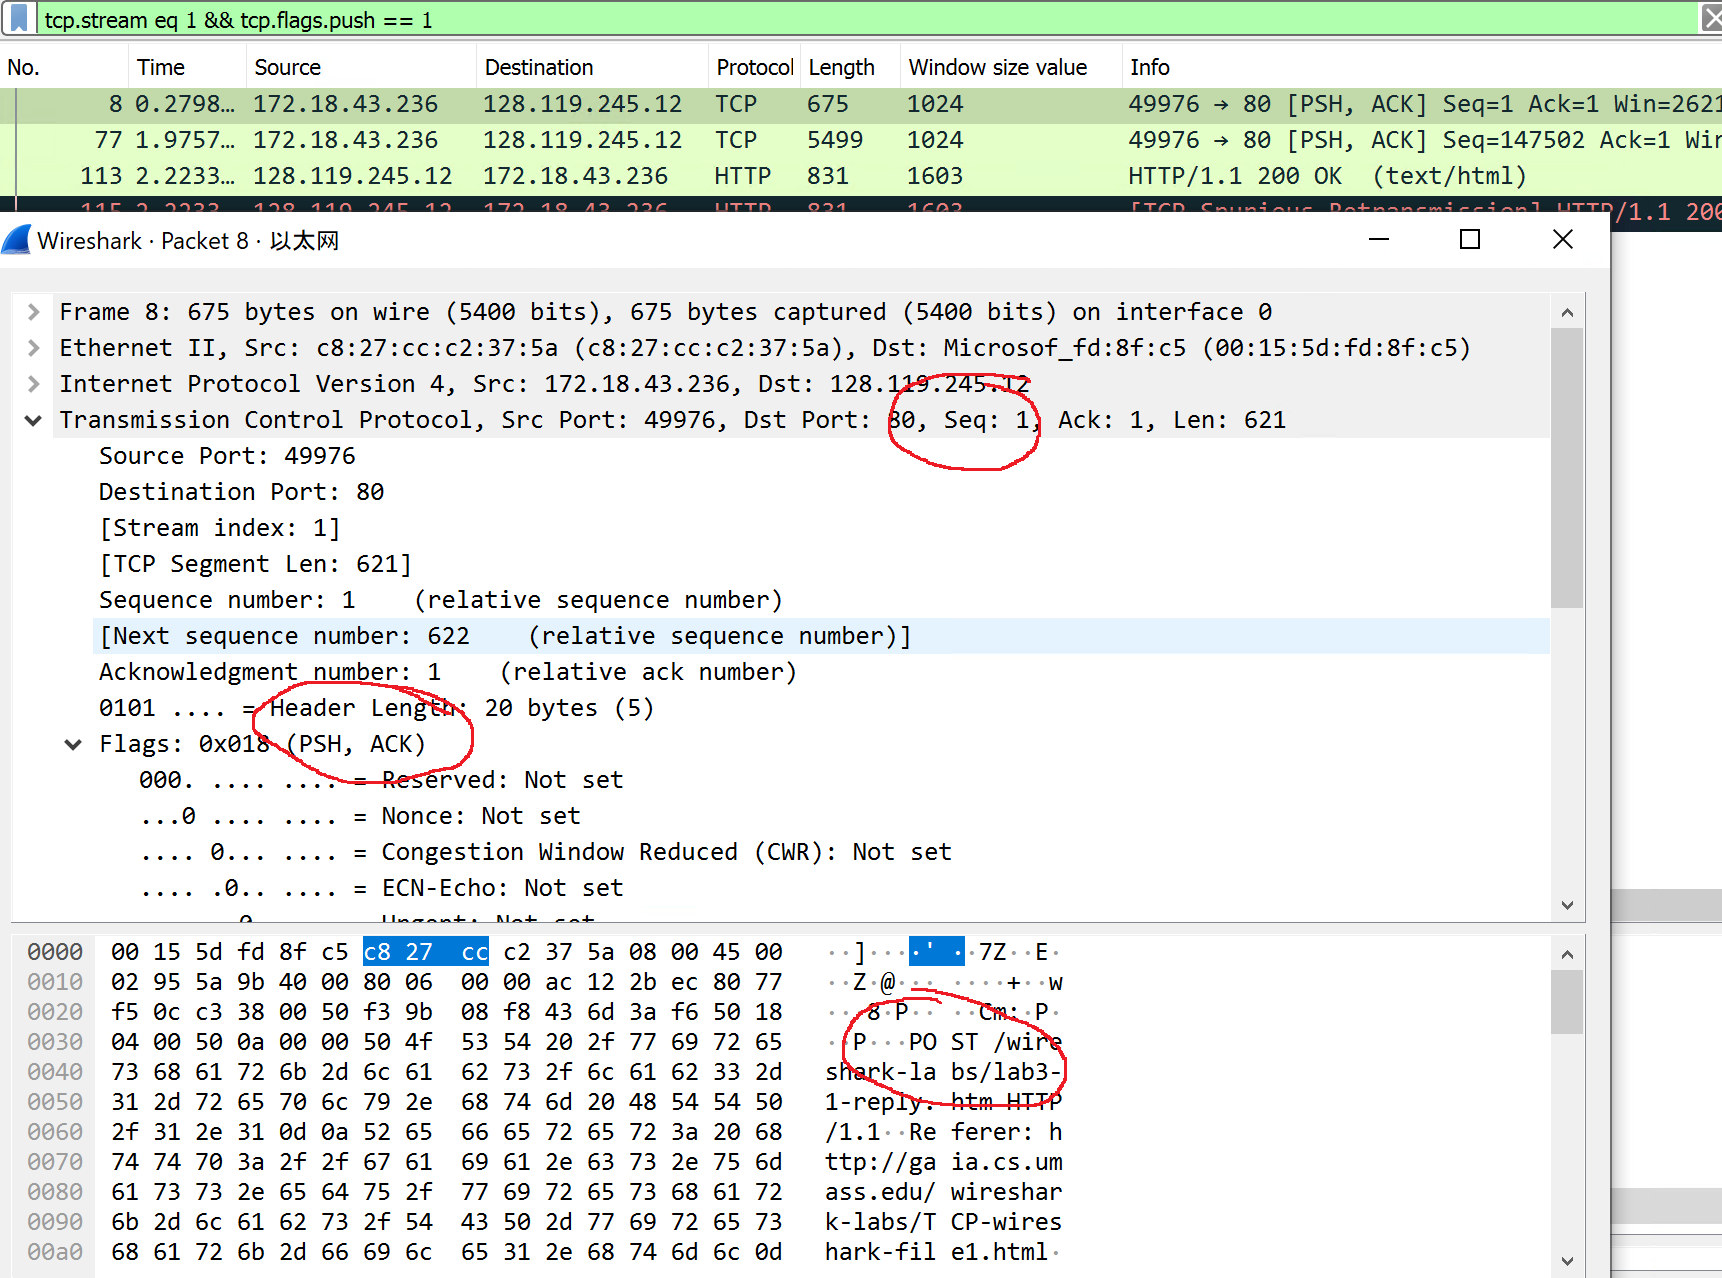
\includegraphics[width=\linewidth]{assets/post.png}
  \caption{HTTP POST request to \href{http://httpbin.org/post}{http://httpbin.org/post}}
  \label{fig:post}
\end{figure}

As packet captured in Figure~\ref{fig:tcp}, the sequence number is 1.

\section*{Problem 7.2.7}
{\bf Description}

Consider the TCP segment containing the HTTP POST as the first segment in the TCP connection.
What are the sequence numbers of the first six segments in the
TCP connection (including the segment containing the HTTP POST)?
At what time was each segment sent?  When was the ACK for each segment received?
Given the difference between when each TCP segment was sent, and when its acknowledgement was received, what is the RTT value for each of the six segments?
What is the EstimatedRTT value (see Section 3.5.3, page 242 in text) after the receipt of each ACK?
Assume that the value of the EstimatedRTT is equal to the measured RTT for the first segment, and then is computed using the EstimatedRTT equation on page 242 for all subsequent segments.

Note: Wireshark has a nice feature that allows you to plot the RTT for each of the TCP segments sent.  Select a TCP segment in the “listing of captured packets” window that is being sent from the client to the gaia.cs.umass.edu server.  Then select: Statistics->TCP Stream Graph>Round Trip Time Graph.

{\bf Solution}


From Figure~\ref{fig:rtt}, we can know

\begin{figure}[H]
  \centering
  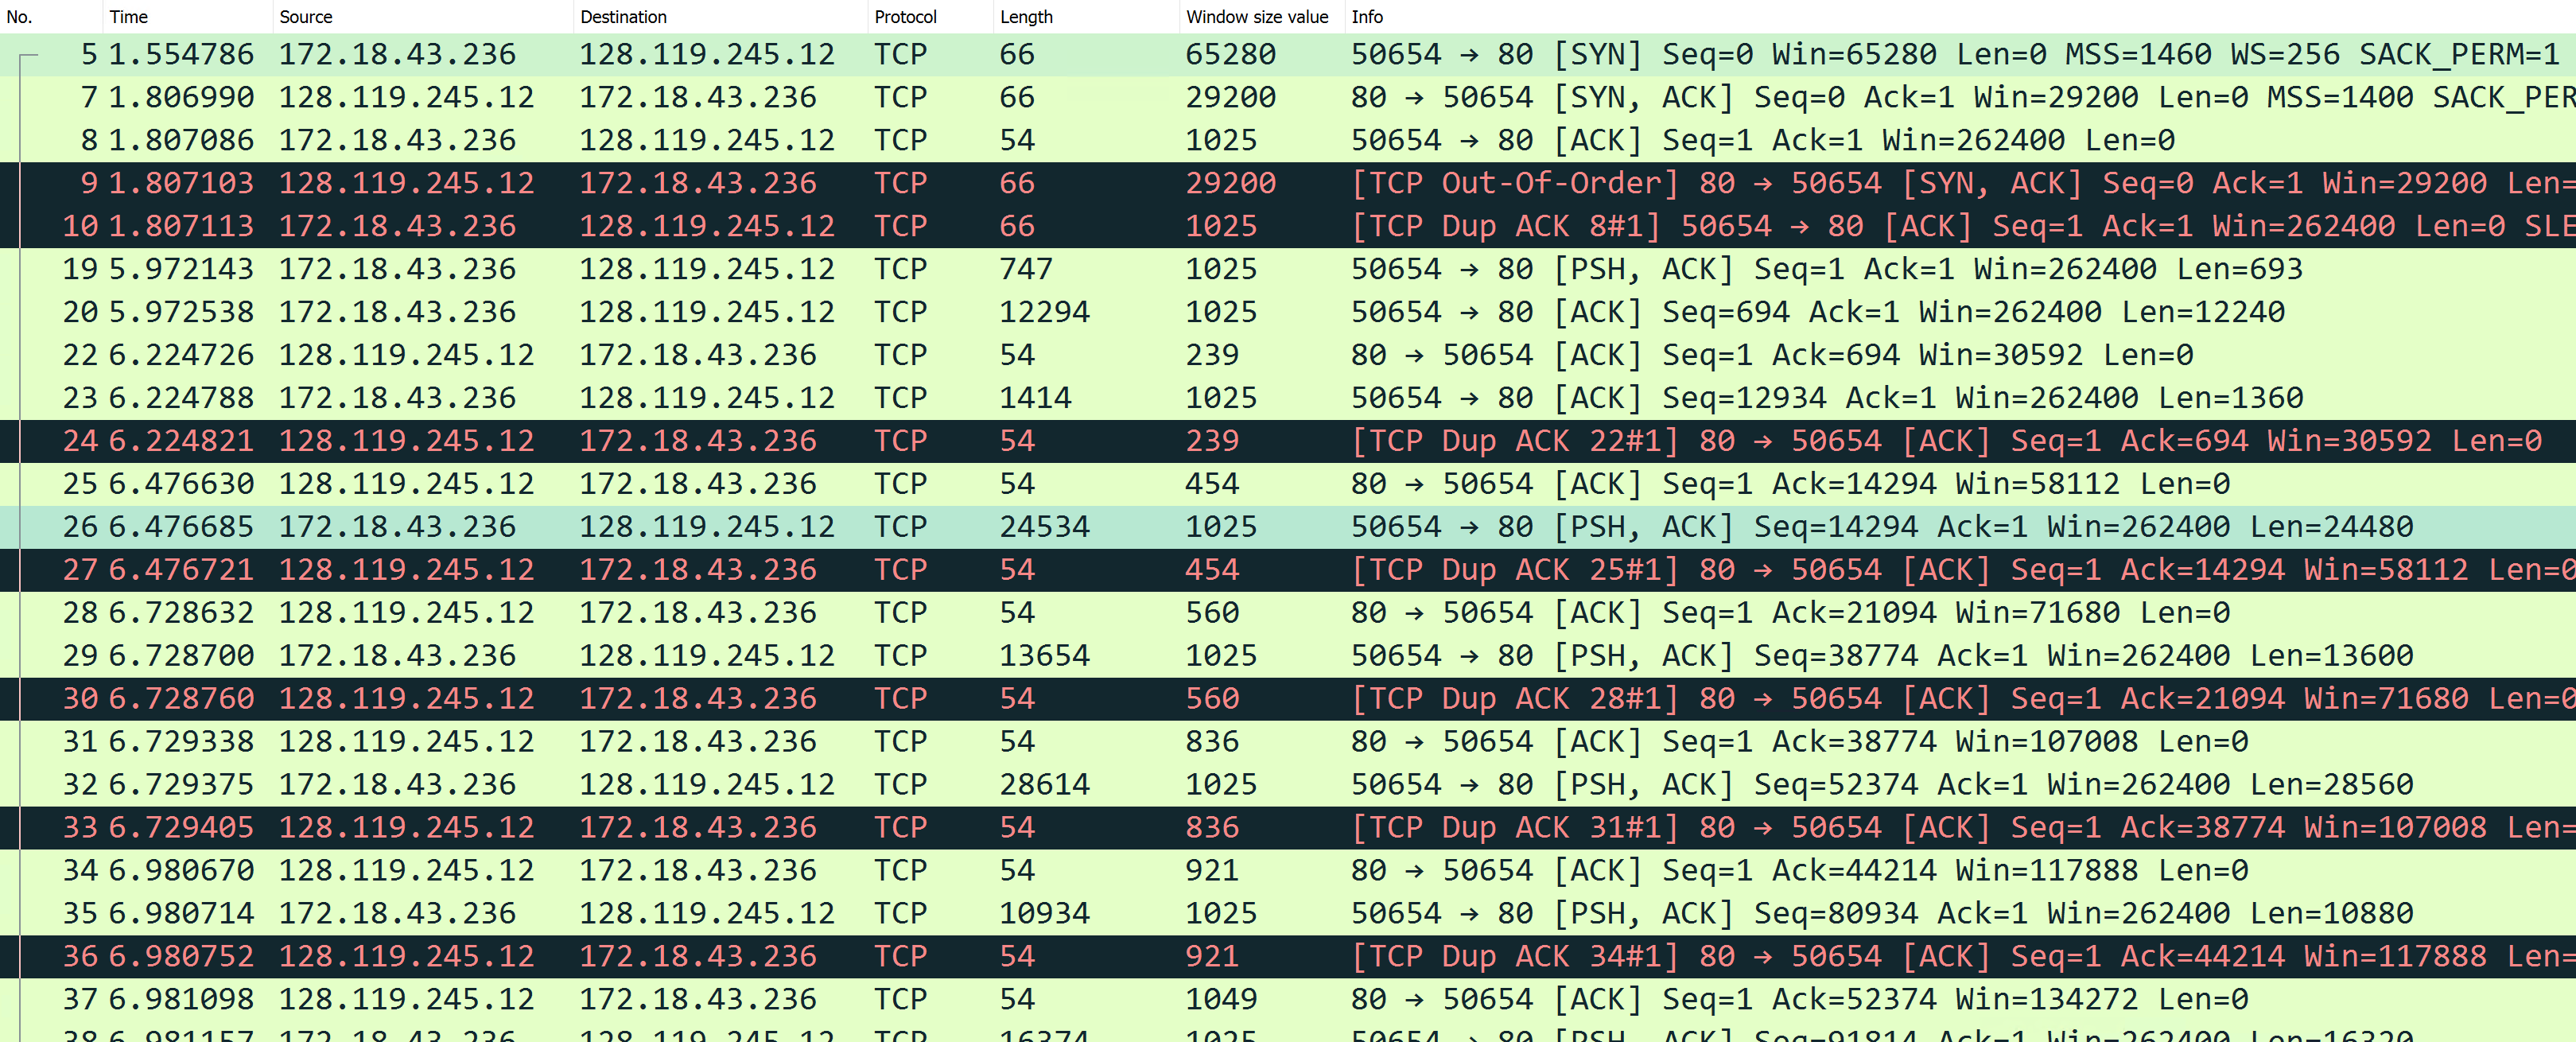
\includegraphics[width=\linewidth]{assets/rtt.png}
  \caption{Upload alice.txt}
  \label{fig:rtt}
\end{figure}

\begin{table}
  \centering
  \caption{Frist 6 Frames}
  \begin{tabular*}{\linewidth}{ccccc}
  \hline
  Num & Seq Number & Start(Sent) & End(Recive ACK)  & RTT \\
  \hline
  1   & 1          & 5.972143s   & 6.224726s        & 0.252583s \\
  2   & 694        & 5.972538s   & 6.224788s        & 0.252250s \\
  3   & 12934      & 6.224788s   & 6.476630s        & 0.251842s \\
  4   & 14294      & 6.476685s   & 6.729338s        & 0.252653s \\
  5   & 38774      & 6.728700s   & 6.981098s        & 0.252398‬s \\
  6   & 52374      & 6.729375s   & 6.981837‬s‬        & 0.252462s \\
  \hline
  \end{tabular*}
\end{table}

$\text{EstimatedRTT} = 0.252583\text{s}$

$\text{EstimatedRTT} = 0.875 * 0.252583\text{s} + 0.125 * 0.252250\text{s} = 0.252541\text{s}$

$\text{EstimatedRTT} = 0.875 * 0.252541\text{s} + 0.125 * 0.251842\text{s} = 0.252454‬\text{s}$

$\text{EstimatedRTT} = 0.875 * 0.252454\text{s} + 0.125 * 0.252653\text{s} = ‭0.252479\text{s}$

$\text{EstimatedRTT} = 0.875 * 0.252479‬‬\text{s} + 0.125 * 0.252398\text{s} = 0.252469\text{s}$

$\text{EstimatedRTT} = 0.875 * 0.252469\text{s} + 0.125 * 0.252462\text{s} = 0.252468\text{s}$


\begin{figure}[H]
  \centering
  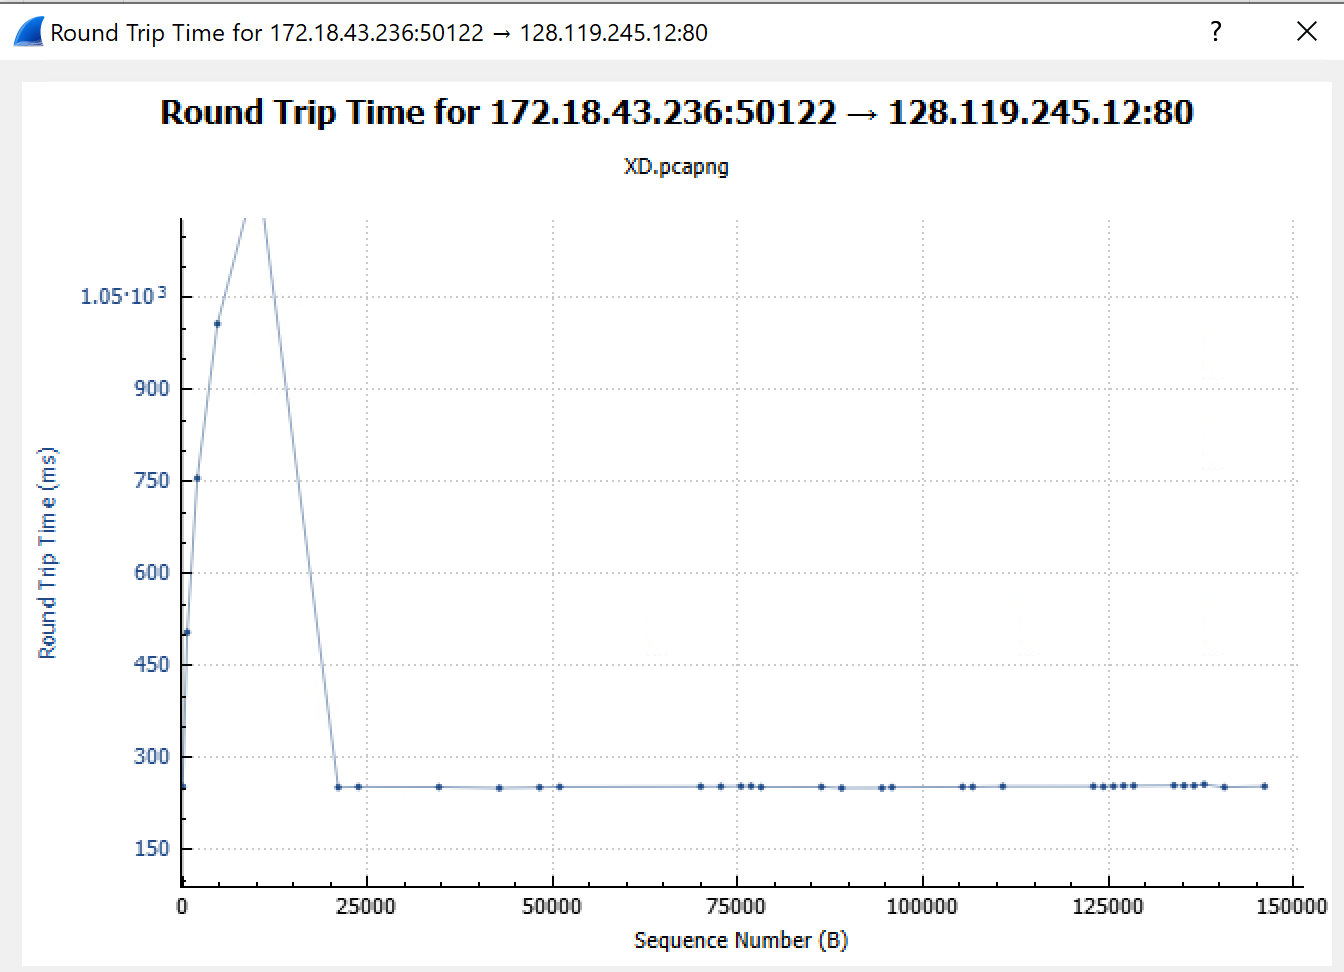
\includegraphics[width=0.7\linewidth]{assets/graph.png}
  \caption{RTT Graph}
  \label{fig:rtt}
\end{figure}

\newpage

\section*{Problem 7.2.9}
{\bf Description}

What is the minimum amount of available buffer space advertised at the received for the entire trace?
Does the lack of receiver buffer space ever throttle the sender?

{\bf Solution}

\begin{figure}[H]
  \centering
  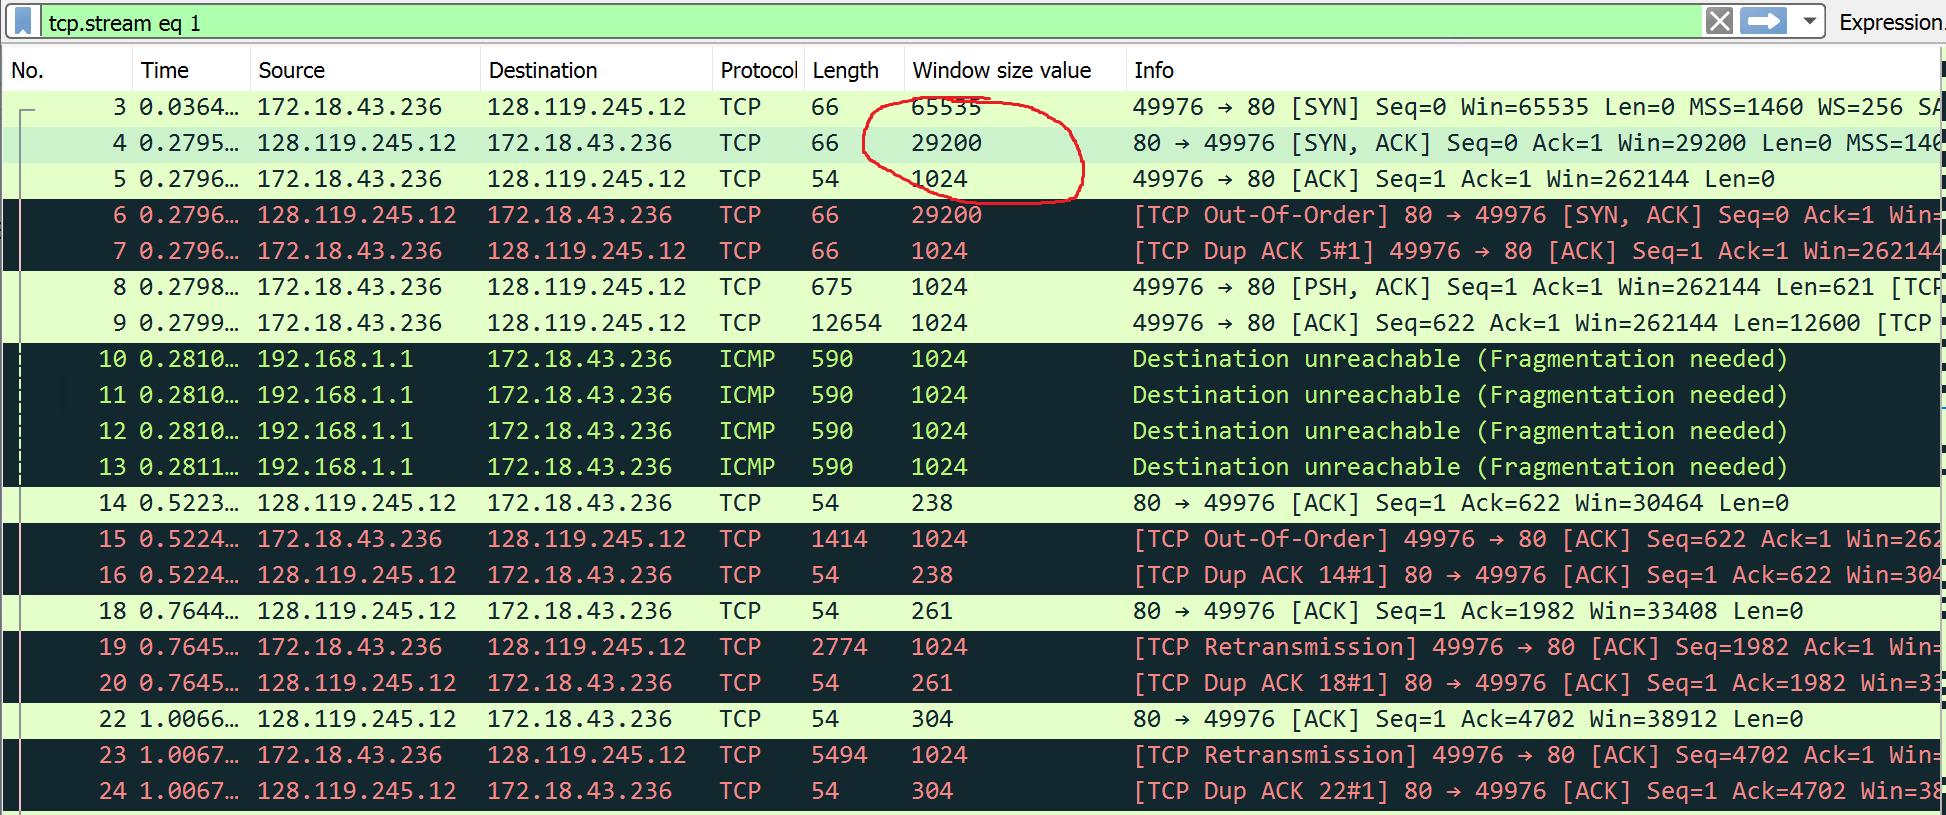
\includegraphics[width=\linewidth]{assets/window.png}
  \caption{Upload alice.txt}
  \label{fig:window}
\end{figure}

As packet captured in Figure~\ref{fig:window}, the minimum amount of available buffer space advertised at the received for the entire trace is 29200.

As Figure~\ref{fig:window_size}, it seems that the reciver buffer space is always enough during this uploading.

\begin{figure}[H]
  \centering
  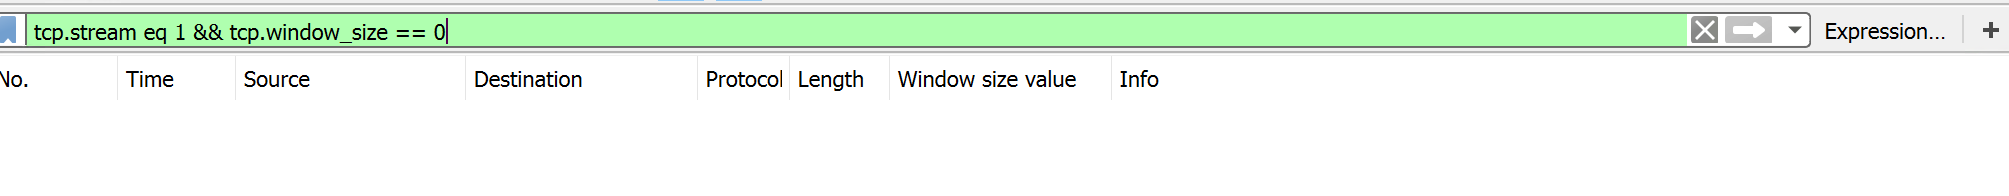
\includegraphics[width=\linewidth]{assets/window_size.png}
  \caption{Confirm there is no such a situation that buffer space is empty}
  \label{fig:window_size}
\end{figure}

\newpage

\section*{Problem 7.2.10}
{\bf Description}

Are there any retransmitted segments in the trace file? What did you check for (in the trace) in order to answer this question?

{\bf Solution}

Yes, there is one retransmitted segment in the trace file. I used filter ``tcp.analysis.retransmissions`` to check for it.

\begin{figure}[H]
  \centering
  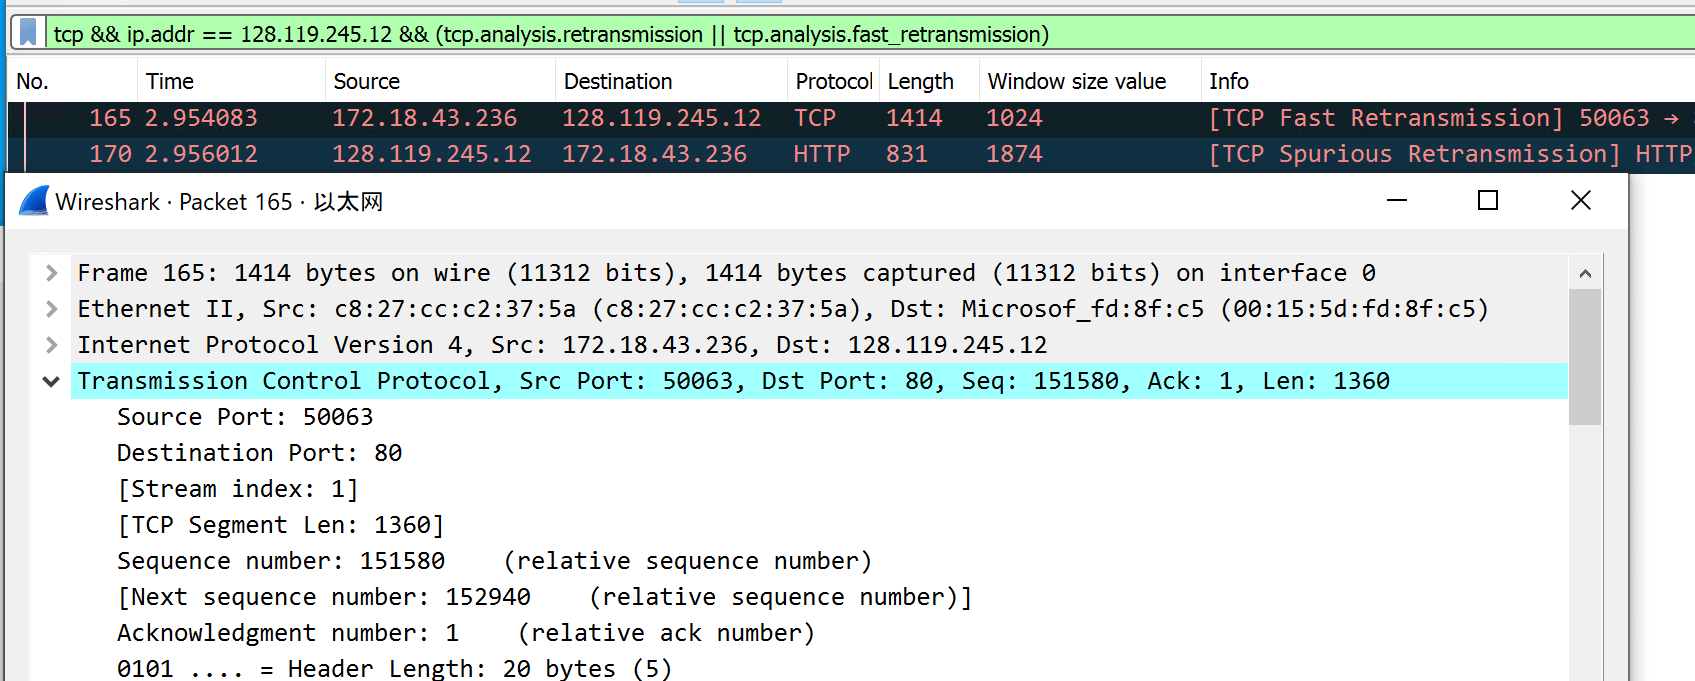
\includegraphics[width=\linewidth]{assets/retransmition.png}
  \caption{Retransmission packets}
  \label{fig:retransmition}
\end{figure}


\newpage

\section*{Problem 7.2.12}
{\bf Description}

What is the throughput (bytes transferred per unit time) for the TCP connection?  Explain how you calculated this value.

{\bf Solution}

The file alice.txt has 152,138 bytes, and download time is $2.954502\text{s} - 1.702976\text{s} = 1.251526\text{s}$.
The throughput of this TCP connection is $\frac{152,138\text{bytes}}{1.251526\text{s}} = 121561.997\text{Bytes/second}$

\begin{figure}[H]
  \centering
  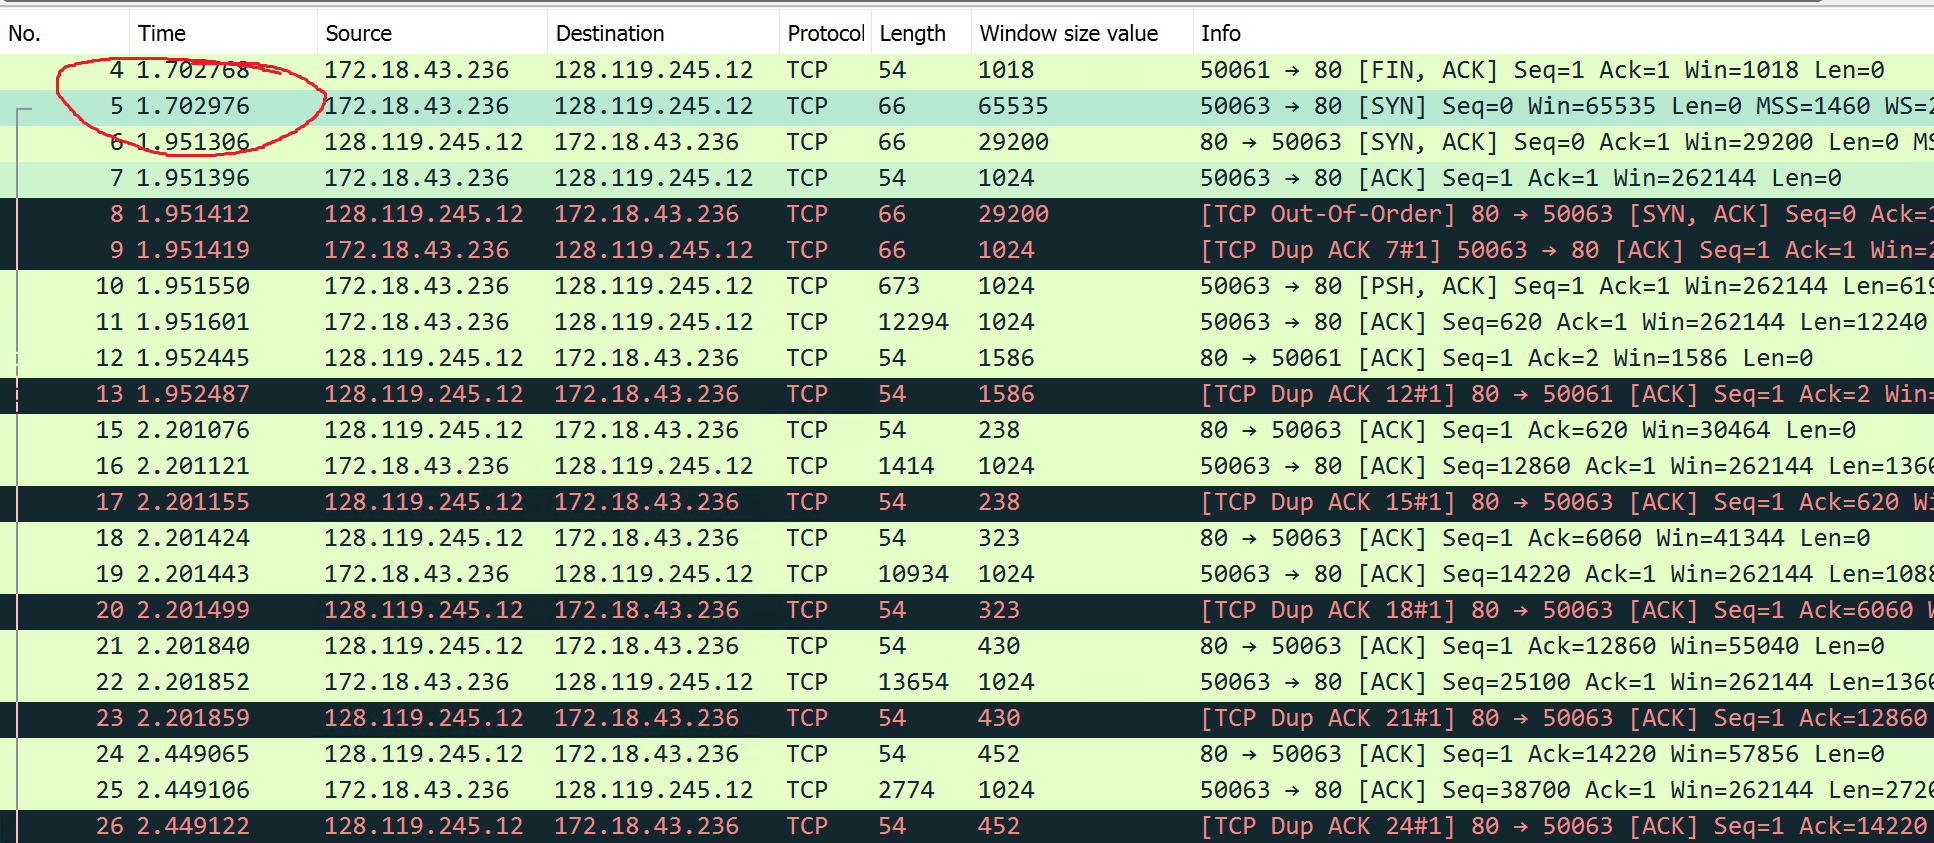
\includegraphics[width=\linewidth]{assets/transmit_1.png}
  \caption{Start transmition at 1.702976s}
  \label{fig:transmit_1}
\end{figure}

\begin{figure}[H]
  \centering
  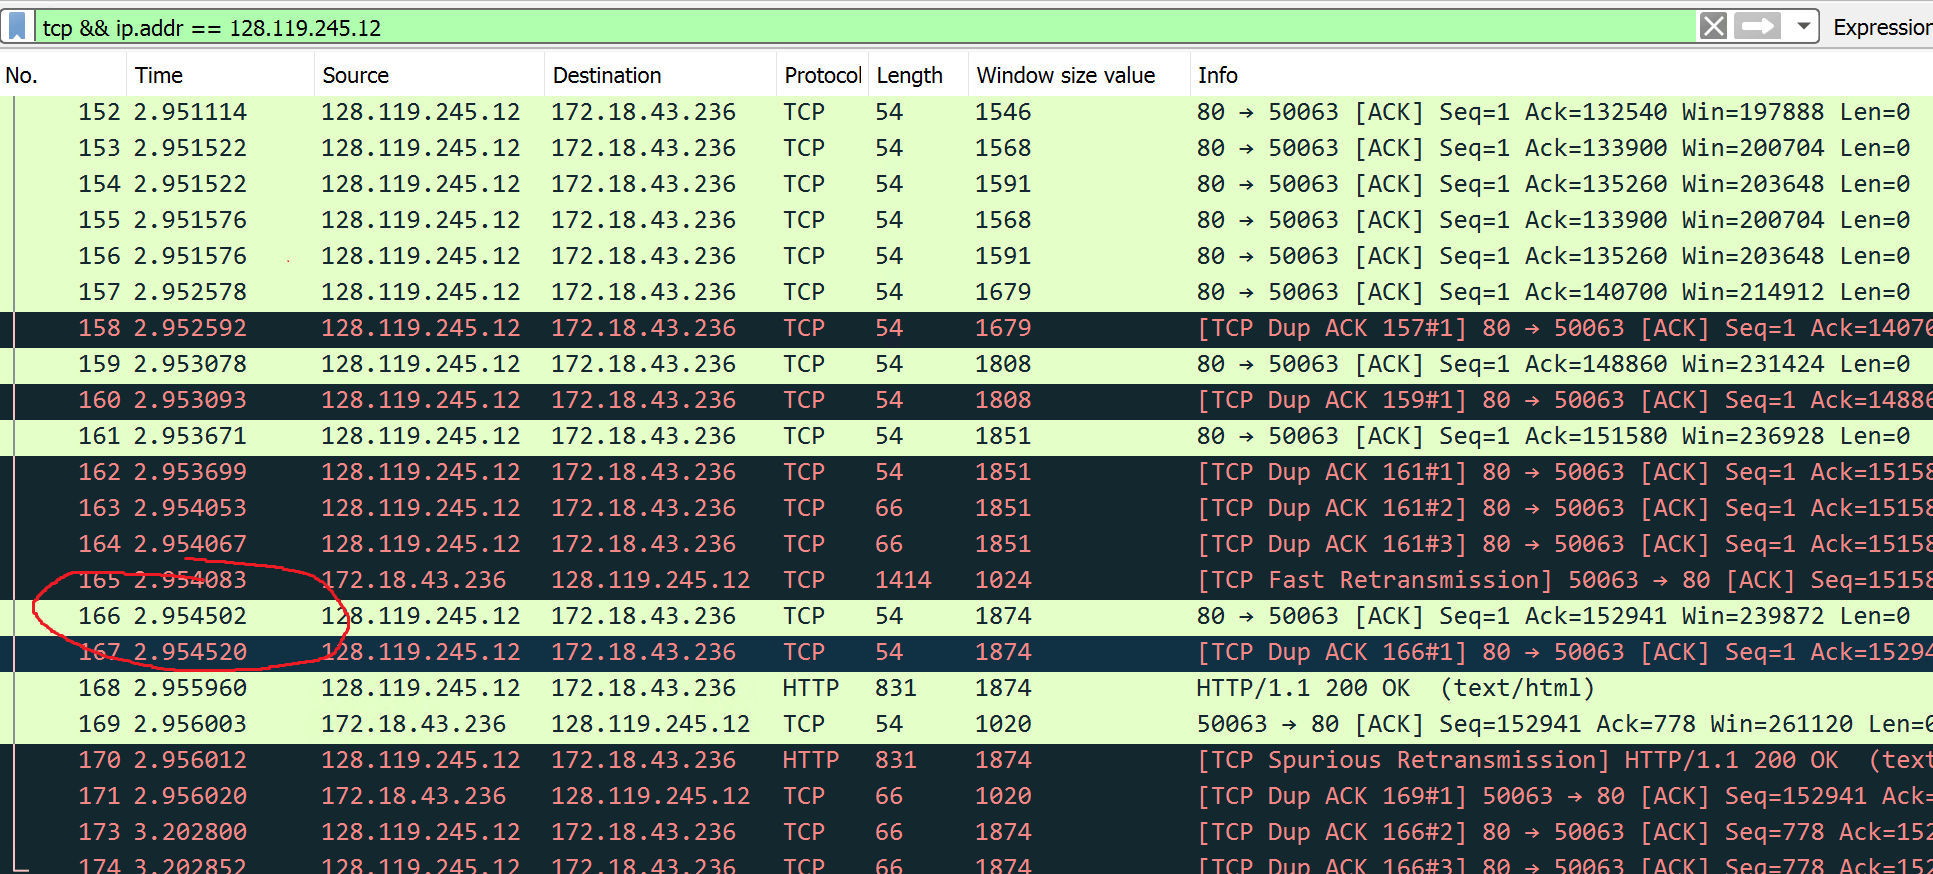
\includegraphics[width=\linewidth]{assets/transmit_2.png}
  \caption{End transmition at 2.954502s}
  \label{fig:transmit_2}
\end{figure}

\end{document}
